This chapter enumerates the steps needed to use one Raspberry Pi Pico to debug
another Raspberry Pi Pico from the command line using OpenOCD and GDB. For
further details refer to the
\href{https://www.raspberrypi.com/documentation/microcontrollers/raspberry-pi-pico.html#debugging-using-another-raspberry-pi-pico}{documentation}.

Note that these instructions are for Linux systems running Debian-based
distributions only. For other operating systems refer to the above link.

\section{Assets}
\begin{enumerate}
    \item Two Raspberry Pi Pico boards.
    \item Female-to-female and Male-to-female jumper wires.
    \item One B-type USB cable.
    \item A laptop running a Debian-based Linux distribution such as Ubuntu. 
\end{enumerate}

\section{Setup}
\begin{enumerate}
    \item Setup the Raspberry Pi Pico environment on your laptop by entering the
    following commands at a terminal window.

    \begin{lstlisting}
sudo apt update && sudo apt upgrade
sudo apt install pkg-config
cd
wget https://raw.githubusercontent.com/raspberrypi/pico-setup/master/pico_setup.sh
chmod +x ./pico_setup.sh
SKIP_VSCODE=1 INCLUDE_PICOPROBE=1 ./pico_setup.sh
    \end{lstlisting}

    \item Download the picoprobe file from this 
    \href{https://www.raspberrypi.com/documentation/microcontrollers/raspberry-pi-pico.html#debugging-using-another-raspberry-pi-pico}{link}.
    \item Connect the Raspberry Pi Pico board to be used as the debugger
    (henceforth referred to as the ``debugger'') to your laptop and
    simultaneously press the BOOTSEL button to boot the debugger in bootloader
    mode.
    \item Flash the downloaded \texttt{picoprobe.uf2} file using
    \texttt{picotool} to the debugger as follows.
    \begin{lstlisting}
picotool save /path/to/picoprobe.uf2
    \end{lstlisting}
    \item Wire the debugger to the other Raspberry Pi Pico board by following
    the wiring diagram in \autoref{fig:picoprobe}.
    \begin{figure}[!ht]
        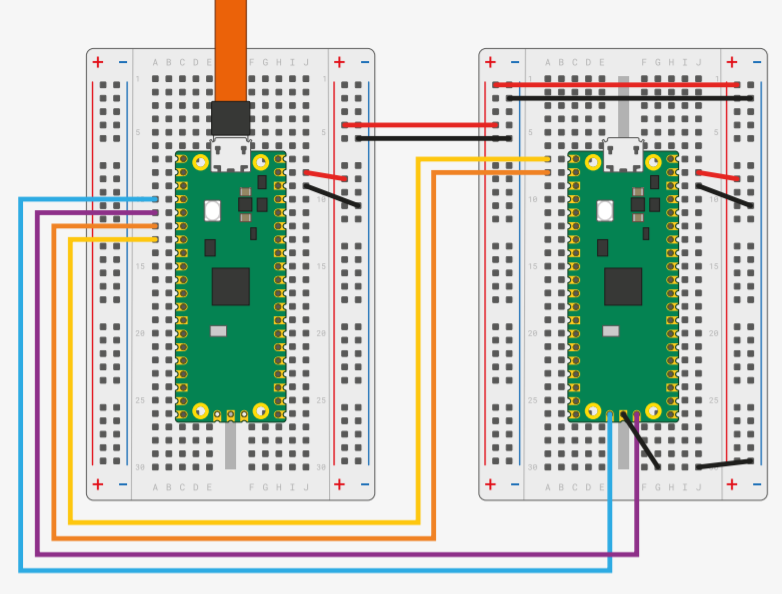
\includegraphics[width=\columnwidth]{picoprobe/figs/picoprobe.png}
        \caption{Wiring diagram to debug a Pico (right) using another Pico as Picoprobe (left).}
        \label{fig:picoprobe}
    \end{figure}
\end{enumerate}

\section{Building}
\begin{enumerate}
    \item Build a debuggable ELF file to load onto the Pico by entering the
    following commands at a terminal window.
    \begin{lstlisting}
cd ~/pico/pico-examples/build
rm -rf ./*
source ~/.bashrc
cmake -DCMAKE_BUILD_TYPE=Debug ..
cd hello_world/serial
make -j4
    \end{lstlisting}
    \item A successful build should generate the debuggable ELF file
    \begin{lstlisting}
~/pico/pico-examples/build/hello_world/serial/hello_serial.elf
    \end{lstlisting}
\end{enumerate}

\section{Debugging}
\begin{enumerate}
    \item Connect the debugger to the laptop again and simultaneously press the
    BOOTSEL button on the target Pico board (and \emph{not} the debugger) to
    boot it in bootloader mode.
    \item In a terminal window, start an OpenOCD server by entering the
    following commands.
    \begin{lstlisting}
cd ~/pico/openocd
sudo src/openocd -f tcl/interface/cmsis-dap.cfg -f tcl/target/rp2040.cfg -s tcl -c "adapter speed 5000"
    \end{lstlisting}
    A successful execution of these commands will result in the following
    (truncated) output.
    \begin{lstlisting}
Info: Listening on port 3333 for gdb connections
    \end{lstlisting}
    \item In \emph{another} terminal window, start \texttt{gdb} with the ELF
    file as follows.
    \begin{lstlisting}
cd ~/pico/pico-examples/build/hello_world/serial
gdb-multiarch hello_serial.elf
(gdb) target remote localhost:3333
(gdb) monitor reset init
(gdb) break main
(gdb) continue
    \end{lstlisting}
    Here, you should see the source code for the program flashed onto the target
    Pico.

    \emph{(Optional)} You can also use \texttt{tmux} instead of two separate
    terminal instances.
    \item You can execute instruction by instruction by typing \texttt{next} at
    the GDB prompt. Alternatively, you can step into functions called from the
    main function by \texttt{step}. 
    \item To reset to the start of the program and reach the main breakpoint
    again, type the following.
    \begin{lstlisting}
(gdb) monitor reset init
(gdb) continue
    \end{lstlisting}
    To quit from gdb, type the following.
    \begin{lstlisting}
(gdb) quit
    \end{lstlisting}
    For other functionalities type \texttt{help} at the GDB
    prompt.
    \item To see serial output, attach a terminal to the device by typing the
    following commands at a terminal window.
    \begin{lstlisting}
sudo minicom -D /dev/ttyACM0 -b 115200
    \end{lstlisting}
    Note that if the device is not present at \texttt{/dev/ttyACM0}, then you
    can find the correct port by inspecting the output produced by the
    following command.
    \begin{lstlisting}
sudo dmesg -w
    \end{lstlisting}
\end{enumerate}